\section{Beacon Design}
\fxnote{The following is very \enquote{alpha-release-ish}}

To meet the requirement of extendability, we use a \gls{soa} to design the beacon.
This architecture splits systems into application components, also called services, which are aggregated to make the system as a whole.
These components then serve a single purpose, i.e.\ executes a contained set of logic with a specified outcome.
Communication between components is done through a well-defined protocol, such that no one component is reliant on the inner workings of another;
a component, or service, should be seen as a black box.

This architecture provides a loose coupling in the system, and also allows for easier fault tolerance, since services should be able to be swapped out if they fail.
However, as services needs knowledge about other relevant services, some mechanism for service discovery is typically deployed, this can be a single point of failure.
\fxnote{expand on this and how it can be decentralized}

\subsection{Components of a Beacon}
\label{sub:components_of_a_beacon}
Under the \gls{soa} single instance of a randomness beacon will consist of the following:
\begin{description}
    \item[A number of input collector services] which can collect from a myriad of different sources.
    \item[An input processing service] which aggregates the input from all the collectors.
    \item[A computation service] which commits to the aggregated input, runs the computation to generate an output.
    \item[A number of publishing services] which can publish the commitment, output, and any relevant proofs, to different outlets.
\end{description}

% \begin{figure}[htpb]
%     \centering
%     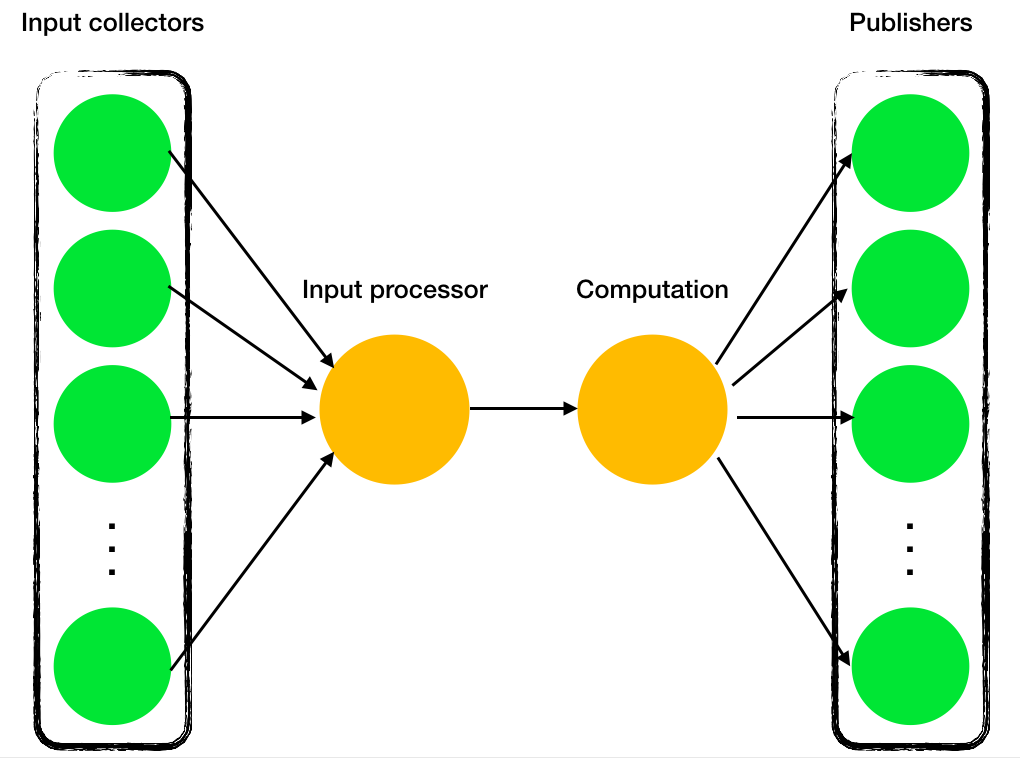
\includegraphics[width=0.98\linewidth]{architecture.png}
%     \caption{Very primitive sketch of architecture}
% \end{figure}
\subimport{}{beacon_architecture.tex}

\subsection{Pipeline}%
\label{sub:pipeline}
Besides the \gls{soa}, we also use a pipeline architecture, to design the beacon.
Data only flows one way through the system, and each component performs an independent transformation.
This effectively means that a beacon is a pipeline, where data flows into the system as inputs, is processed, transformed to a random output, and lastly published.
The pipeline architecture can be seen as a specialization of the \gls{soa} pattern, since each step in the pipeline is a service as defined in a \gls{soa}.

When considering the system as a pipeline, we also get some restrictions compared to a more generic \gls{soa}, in that data only flows in one direction.
Moreover, the pipeline architecture can be used to specify types of components as we did in~\vref{sub:components_of_a_beacon}, these types can then be aggregated according to a specification to define a complete beacon.

The pipeline also allows for parallel operation, i.e.\ input collectors can run continuously as can the computation service.
This effectively means that we can reach the highest possible output of randomness, given a single computation service.
One might argue that several computation services slightly offset in start time, could output more frequently, but this would by our design be considered as several different beacons.

In some scenarios a beacon may consist of multiple computation services, as a mean of redundancy, as long as each computation is run on the same input.
The same can be said about input processors, where a beacon may need redundancy to likewise avoid a single point of failure.
This brings forth the issue of consensus about which input to use\msmnote{out of scope or explain solutions?}.

\subsection{Security Design (Preliminary Security Analysis)}
When designing a composable system such as our randomness beacon, it is important to take into account, the inter component communication.
From a security aspect, splitting up the system from a monolithic self contained architecture to a service oriented kind, exposes a myriad of new attack surfaces.
For example this architecture can potentially make it possible for adversaries to cut off parts of the system, by means of \gls{dos} attacks.
Moreover the protocol used to communicate from service to service, must be secure in a way that prevents adversaries from being able to undetectably manipulate the messages.

\mtjnote{Mention Slow Hashing functions here}

\mtjnote{Comparison with Drand}

\mtjnote{The beacon is secure because:}
The operator does not know the individual inputs before receiving them
He commits to using the inputs, i.e.\ he cannot change the order of them to his own benefit.
What keeps him from trying out multiple commitments before publishing one?
The slow hash function ensures that he cannot try excessively many commitments.
